\documentclass[12pt]{article}

\usepackage[margin=1in]{geometry} 
\usepackage{amsmath,amsthm,amssymb}
\usepackage[spanish]{babel}
\usepackage[utf8]{inputenc}
\usepackage{tikz-cd}
\usepackage{amsmath}
\usepackage[shortlabels]{enumitem}
\usepackage{mathtools}
\usepackage{float}
\usepackage{listings}

\begin{document}

\title{SWAP: Ejercicio T4.4}
\author{
        Antonio Gámiz Delgado
}
\maketitle
\medskip

Vamos a instalar \textit{Zevenet}. Primero preparamos nuestro host y descargamos la imagen docker necesaria de \cite{a1}, con los comandos:

\begin{figure}[H]
  \center
  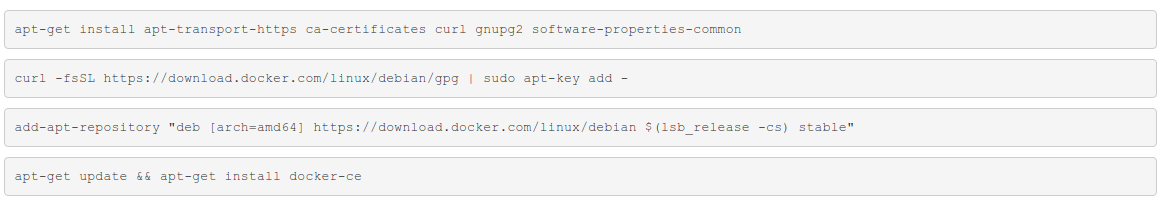
\includegraphics[scale=0.5,width=\textwidth]{img/2.png}
  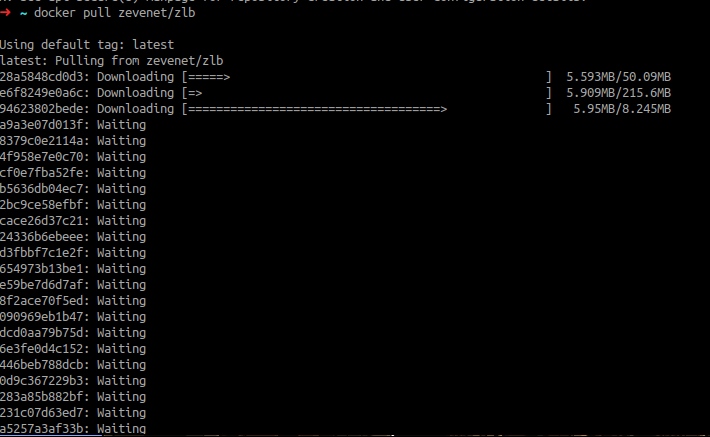
\includegraphics[scale=0.5,width=\textwidth]{img/3.png}
\end{figure}

Una vez descargada, ponemos en marcha el contenedor:

\begin{figure}[H]
  \center
  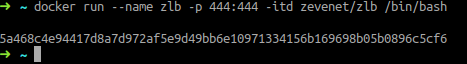
\includegraphics[scale=0.5,width=\textwidth]{img/4.png}
\end{figure}

Y abrimos la interfaz gráfica en el navegador:

\begin{figure}[H]
  \center
  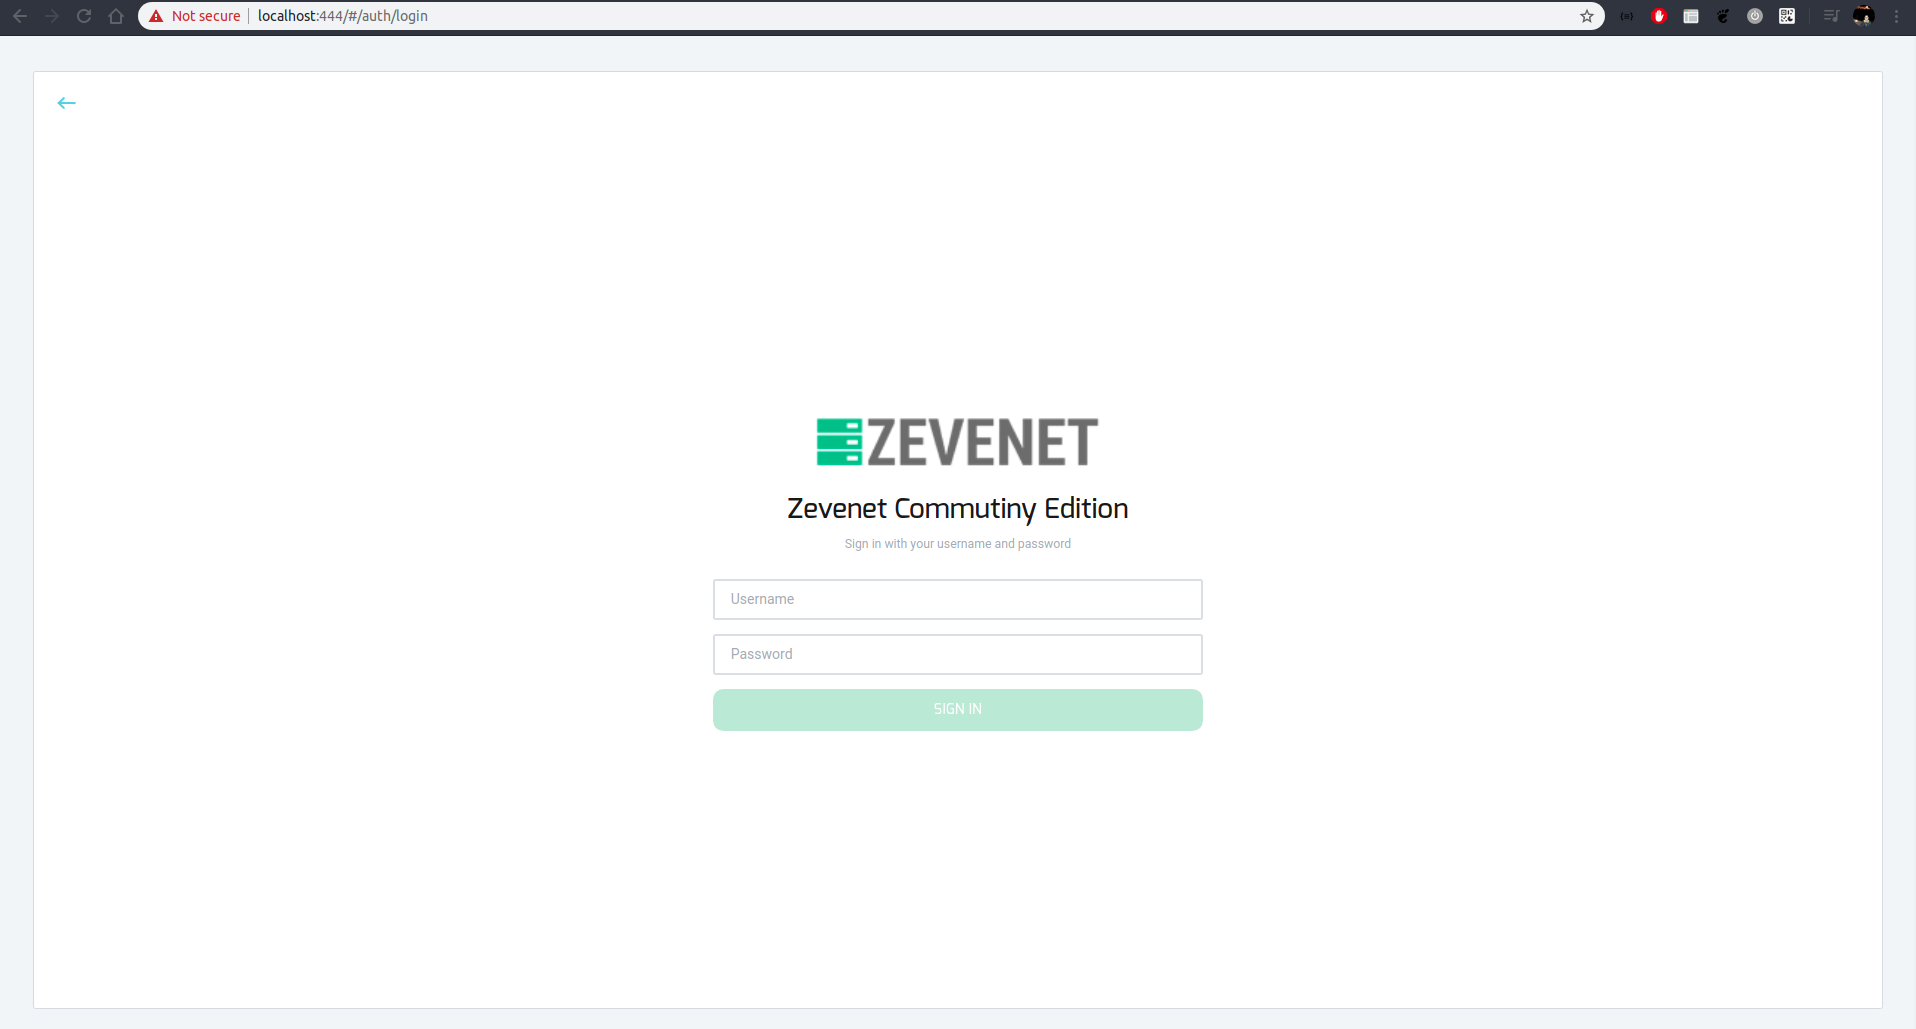
\includegraphics[scale=0.5,width=\textwidth]{img/5.png}
\end{figure}

Y aquí me he quedado atascado básicamente. Me he registrado y no me deja hacer login, he intentado también instalarlo mediante la ISO pero tampoco me ha dejado. Conclusión: hes muy difícil de instalar, la documentación deja bastante que desear y ni siquiera las páginas para hacer login funcionan.

\begin{thebibliography}{9}
\bibitem{paginaofic22ial}
https://www.zevenet.com/es/
\bibitem{instalacion}
https://www.zevenet.com/knowledge-base/community-edition/community-edition-v5-0-administration-guide/ce-v5-0-installation-guide/
\bibitem{a1}
https://www.zevenet.com/knowledge-base/community-edition/dockerizing-zevenet-ce/
\bibitem{a2}
https://www.zevenet.com/es/base-de-conocimientos/edici\%C3\%B3n-comunitaria/Edici\%C3\%B3n-de-la-comunidad-v3-05-gu\%C3\%ADa-de-administraci\%C3\%B3n/comunidad-edici\%C3\%B3n-v3-05-granjas-de-perfiles-http/
\end{thebibliography}

%\begin{figure}[H]
%  \center
%  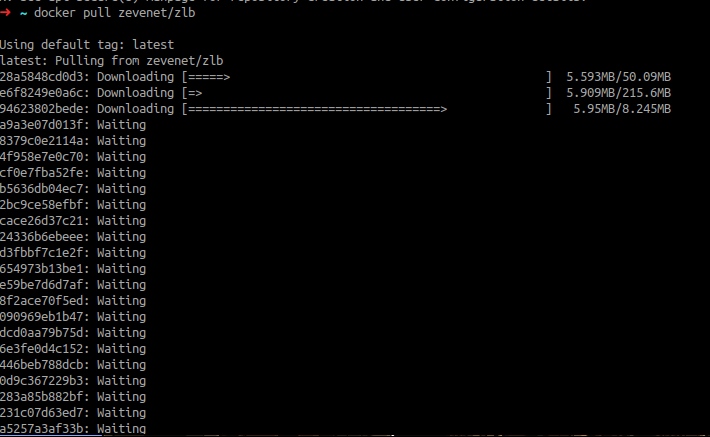
\includegraphics[scale=0.5]{img/3.png}
%\end{figure}

\end{document}
